\documentclass[12pt,a4paper]{report}

% ------------------------------------------------
% Packages
% ------------------------------------------------

\usepackage[a4paper,margin=1in]{geometry}
\usepackage[T1]{fontenc}
\usepackage{newtxtext,newtxmath}
\usepackage{setspace}
\usepackage{enumitem}
\usepackage{booktabs}
\usepackage{array}
\usepackage{longtable}
\usepackage{graphicx}
\usepackage{float}
\usepackage{caption}
\usepackage[hidelinks]{hyperref}
\usepackage{fancyhdr}

\setstretch{1.12}

\setlength{\parindent}{0pt}
\setlength{\parskip}{6pt}

% ------------------------------------------------
% Header / Footer
% ------------------------------------------------

\pagestyle{fancy}
\fancyhf{}
\fancyfoot[C]{\thepage}
\renewcommand{\headrulewidth}{0pt}

% ------------------------------------------------
% Document
% ------------------------------------------------

\begin{document}

% =================================================
% TITLE PAGE
% =================================================

\begin{titlepage}

\centering

\vspace*{0.8in}

{\Large\bfseries UCS503 -- Software Engineering\par}

\vspace{0.3in}

{\LARGE\bfseries Smart City Civic Complaint and Management System\par}

\vspace{0.25in}

{\large A Web-Based Platform for Civic Complaint Registration,
Tracking and Resolution\par}

\vspace{0.8in}

\textbf{Submitted by:}\par

\vspace{0.15in}

1024170429 Achintya Maurya\par
1024170437 Hittin Gupta\par




\vspace{0.3in}

\textbf{Group: 3Q41 BE Third Year, CSE}\par

\textbf{BE Third Year, CSE}\par

\vspace{0.6in}

\textbf{Submitted to:}\par

\vspace{0.15in}

Dr. Nisha Thakur\par

Computer Science and Engineering Department\par

Thapar Institute of Engineering and Technology, Patiala\par

\vfill

\textbf{Mid-Semester Evaluation}\par

September 2026

\end{titlepage}


% =================================================
% CHAPTER 1
% =================================================

\chapter{Introduction}

\section{Background and Context}

Urban areas generate a large number of civic complaints related to roads, street lights, sanitation, drainage, waste management, public infrastructure, and other municipal services. In a conventional complaint-management process, citizens may have limited visibility into the status of their complaints after submitting them. Complaints can also require coordination between different departments and field-level workers before the reported issue is resolved.

The Smart City Civic Complaint and Management System is proposed as a web-based platform that provides a structured process for registering, managing, tracking, and resolving civic complaints. The system connects citizens with department officers and field workers through a centralized workflow.

A citizen can register or log in to the system, submit a complaint by providing relevant details and location information, and optionally upload a photograph as supporting evidence. The system generates a unique complaint ID and maintains the complaint information for further processing.

After submission, the department officer can review and verify the complaint and assign an appropriate field worker. The field worker can view the assigned task, accept the work, update its progress, upload evidence, and mark the work as completed. The citizen can subsequently verify whether the reported issue has been resolved.

The system therefore establishes a complete complaint lifecycle from submission to resolution and citizen verification. The project also considers smart assistance features such as complaint classification, duplicate detection, and priority calculation as planned extensions to the core system.


\subsection{Problem Statement}

The existing complaint-handling process can involve several disconnected activities such as complaint registration, department assignment, field-level work, status updates, and resolution verification. Without a centralized system, it can be difficult for citizens to track complaints and for responsible personnel to maintain a consistent record of complaint progress.

The specific problem addressed by this project is the lack of a structured and traceable platform for managing the complete lifecycle of civic complaints.

The proposed system aims to provide:

\begin{itemize}[leftmargin=*]

\item A centralized platform for registering civic complaints.

\item A structured mechanism for recording complaint details and location.

\item Unique identification of every submitted complaint.

\item Assignment of verified complaints to appropriate department officers and field workers.

\item Continuous status updates during complaint resolution.

\item Uploading of photographs and work evidence.

\item Citizen verification of the completed work.

\item An option to reopen a complaint when the issue has not been properly resolved.

\item A foundation for future smart features such as classification, duplicate detection, and priority calculation.

\end{itemize}


\section{Project Objectives}

The major objectives of the Smart City Civic Complaint and Management System are:

\begin{enumerate}[leftmargin=*]

\item To develop a centralized web-based platform through which citizens can register and submit civic complaints.

\item To provide a structured complaint workflow covering complaint submission, verification, worker assignment, work progress, resolution, and citizen verification.

\item To maintain complaint information such as category, description, location, photographs, status, and resolution details in an organized manner.

\item To allow department officers to review complaints, verify their validity, assign field workers, and monitor complaint progress.

\item To allow field workers to view assigned tasks, update work progress, upload work evidence, and mark tasks as completed.

\item To provide citizens with complaint tracking and resolution verification functionality.

\item To design the system in an incremental manner so that advanced features such as smart classification, duplicate detection, and priority calculation can be incorporated in later stages.

\item To maintain a traceable record of the complaint lifecycle from initial submission to final closure.

\end{enumerate}


% =================================================
% CHAPTER 2
% =================================================

\chapter{Methodology and Design}

\section{System Architecture}

The Smart City Civic Complaint and Management System follows a modular web-based architecture in which different users interact with the system according to their responsibilities.

The major participants in the system are:

\begin{itemize}[leftmargin=*]

\item \textbf{Citizen:} Registers or logs in, submits complaints, tracks complaint status, verifies resolution, provides feedback, and can reopen an unresolved complaint.

\item \textbf{Department Officer:} Reviews and verifies complaints, assigns field workers, monitors progress, and manages complaint status.

\item \textbf{Field Worker:} Views assigned tasks, accepts work, performs the required work, updates progress, uploads evidence, and marks the work as completed.

\item \textbf{Administrator:} Manages users, departments, workers, and overall complaint information.

\end{itemize}

The system is designed around a central complaint-management workflow. Complaint information submitted by a citizen is processed by the system and subsequently handled by the department officer and field worker.

The general workflow is:

\[
\text{Citizen}
\rightarrow
\text{Complaint Submission}
\rightarrow
\text{Officer Verification}
\rightarrow
\text{Worker Assignment}
\rightarrow
\text{Work Execution}
\rightarrow
\text{Resolution}
\rightarrow
\text{Citizen Verification}
\]

This architecture provides a clear separation of responsibilities between the different actors while maintaining a common complaint lifecycle.


\subsection{High-Level Design}

At a high level, the system can be divided into the following functional components:

\begin{enumerate}[leftmargin=*]

\item \textbf{Citizen Interface}

The citizen interface provides functionality for registration/login, complaint submission, entering complaint details, providing location information, uploading photographs, tracking complaint status, and verifying resolution.

\item \textbf{Complaint Management Layer}

This layer manages the complaint lifecycle. It handles complaint registration, generation of complaint IDs, status management, verification, assignment, and closure.

\item \textbf{Department Officer Module}

The department officer module provides functionality for reviewing complaints, verifying their validity, assigning field workers, and monitoring the progress of complaints.

\item \textbf{Field Worker Module}

The field worker module allows workers to view assigned tasks, accept work, update progress, upload work evidence, and mark work as completed.

\item \textbf{Administration Module}

The administration module is responsible for managing users, departments, workers, and overall complaint monitoring.

\item \textbf{Smart Assistance Layer}

The proposed smart assistance layer contains planned features such as smart classification, duplicate detection, and priority calculation. These features are intended to be introduced after the core complaint workflow is stable.

\end{enumerate}


% ------------------------------------------------
% USE CASE DIAGRAM
% ------------------------------------------------



\subsubsection*{Use Case Diagram}

The Use Case Diagram represents the major actors of the system and the
functions available to each actor. It establishes the functional boundary of
the proposed system and shows the interaction between citizens, department
officers, field workers, administrators, and the system.

\begin{figure}[H]
    \centering
    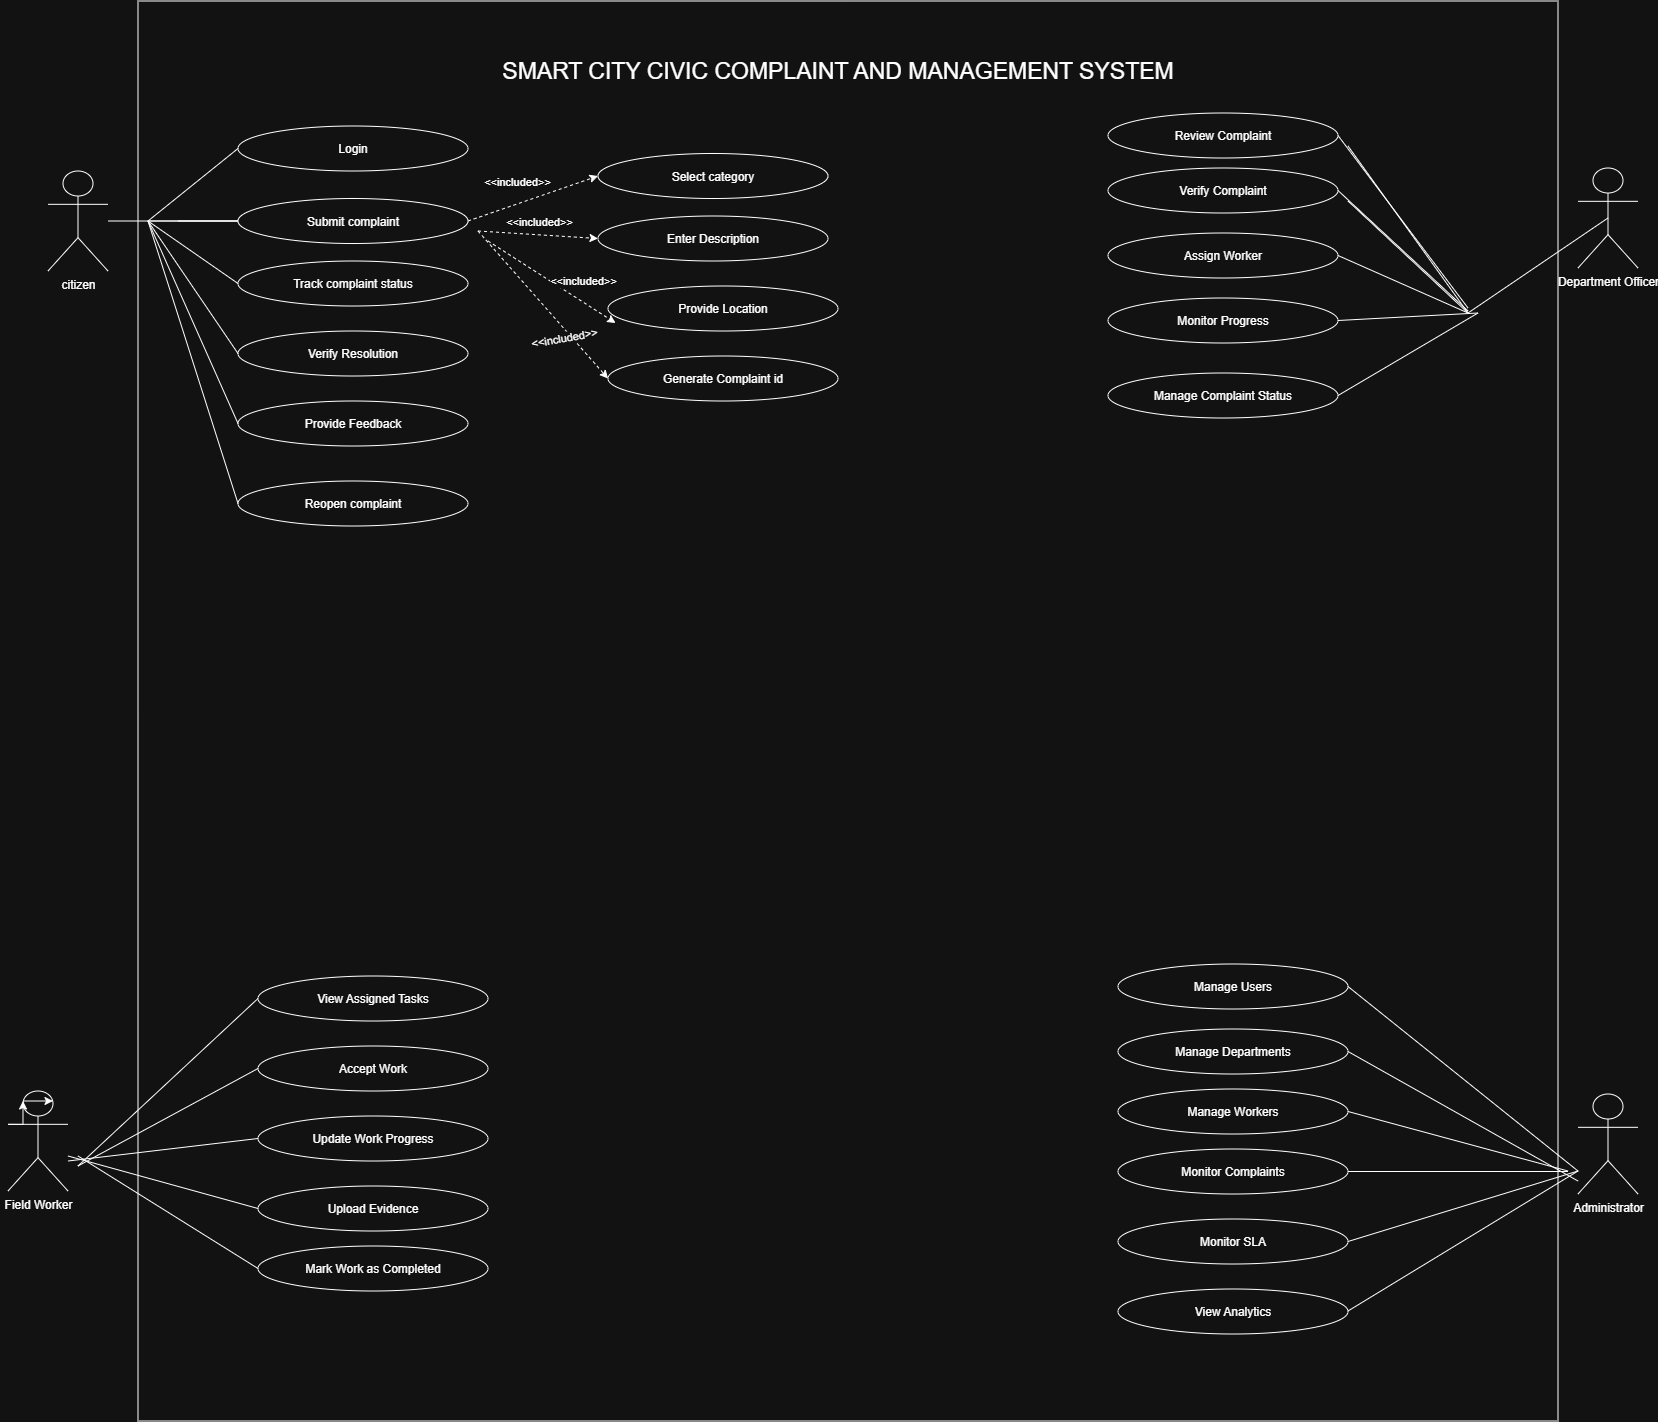
\includegraphics[width=0.90\textwidth]{../assets/Use_case.drawio.png}
    \caption{Use Case Diagram of the Smart City Civic Complaint and Management System}
    \label{fig:usecase}
\end{figure}

The diagram identifies four primary actors: Citizen, Department Officer, Field Worker, and Administrator. The citizen is responsible for complaint creation and verification, the department officer manages verification and assignment, the field worker performs the assigned work, and the administrator manages system-level information.

The diagram also represents the planned smart assistance features including Smart Classification, Duplicate Detection, and Priority Calculation.


% ------------------------------------------------
% ACTIVITY DIAGRAM
% ------------------------------------------------

\subsubsection*{Activity Diagram}


The Activity Diagram represents the complete workflow of the Smart City Civic Complaint and Management System. It shows the sequence of activities starting from citizen login and complaint submission to complaint verification, worker assignment, work completion, and final citizen verification.

\begin{figure}[H]
    \centering
    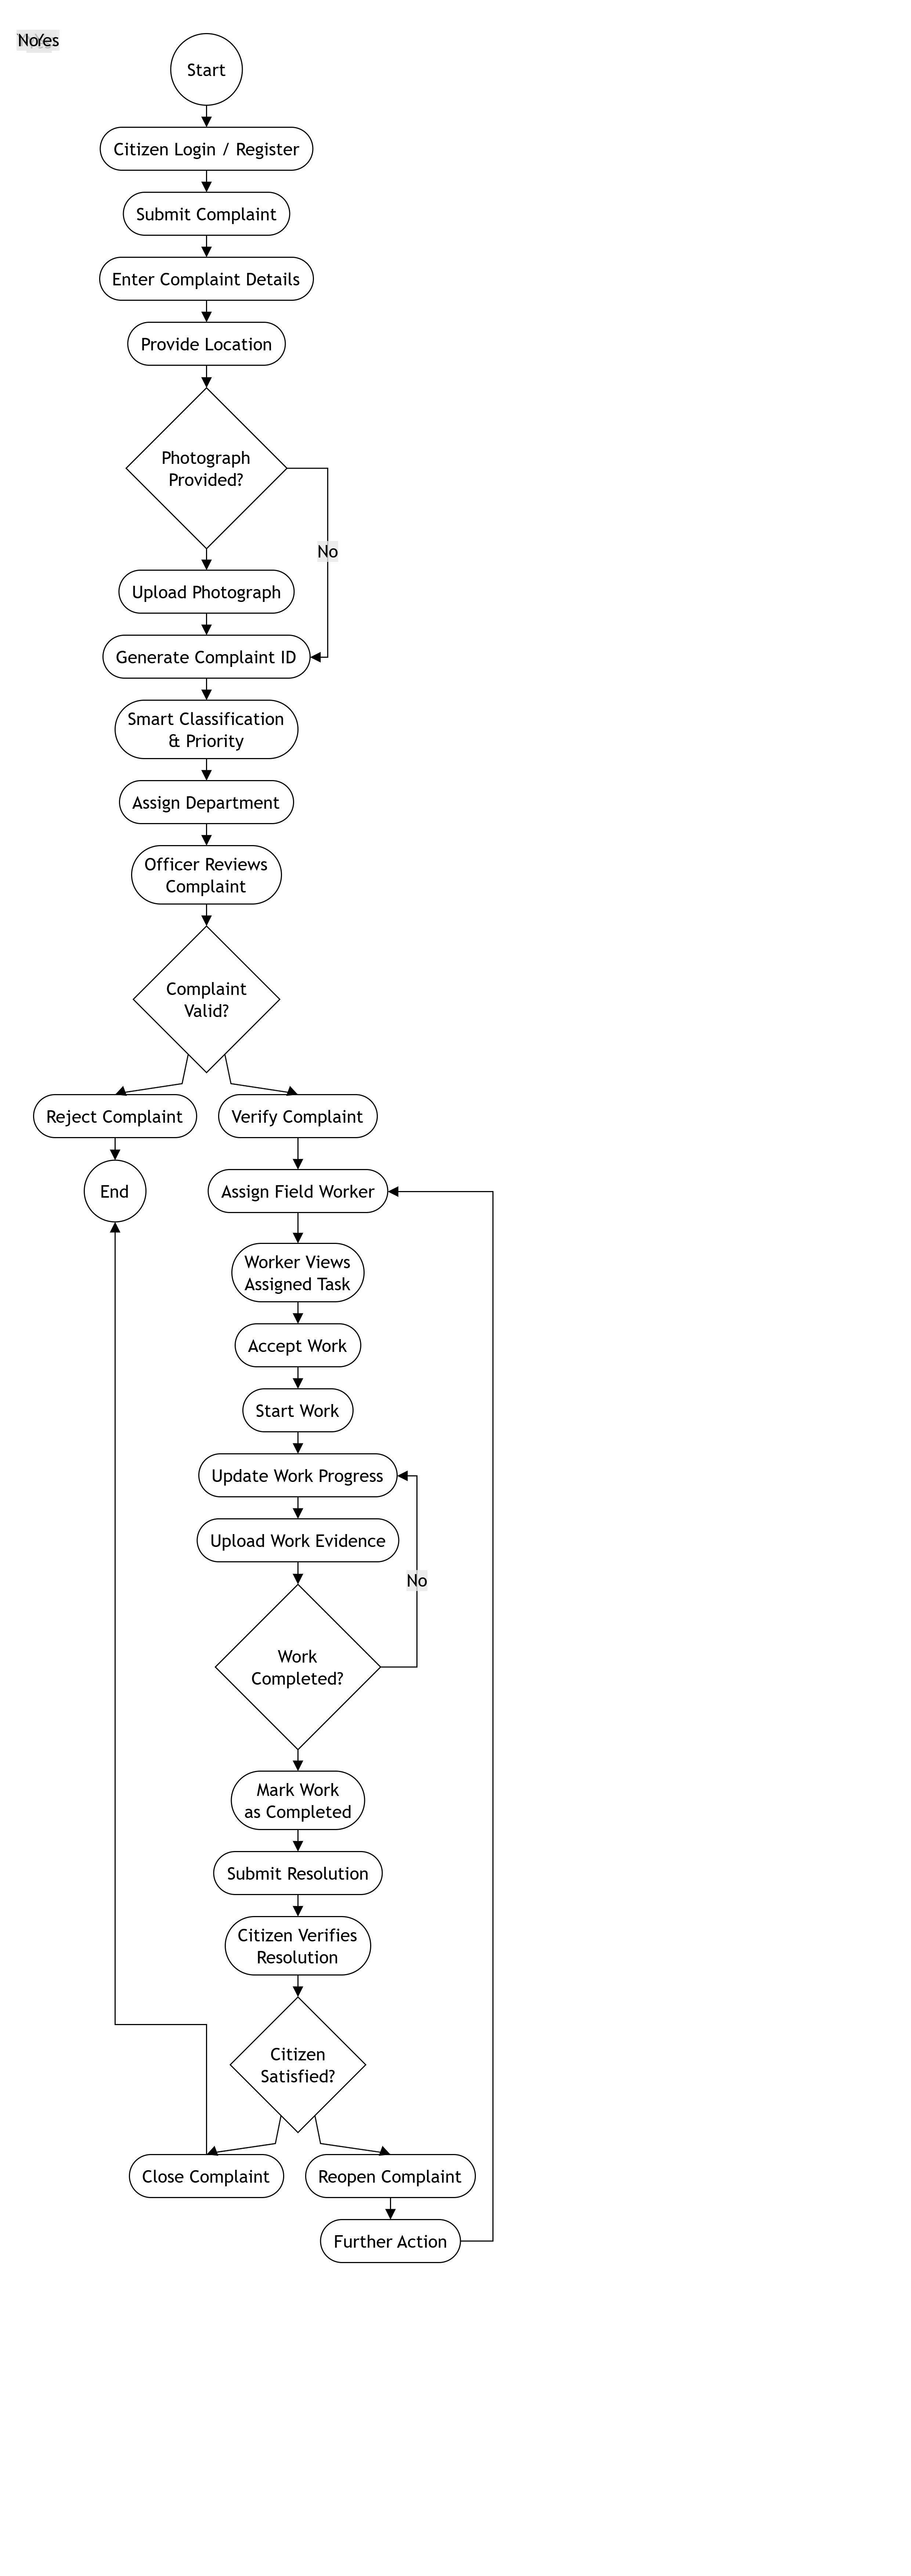
\includegraphics[width=0.70\textwidth]{../assets/activity_diagram.png}
    \caption{Activity Diagram of the Smart City Civic Complaint and Management System}
    \label{fig:activity}
\end{figure}


% ------------------------------------------------
% SEQUENCE DIAGRAM
% ------------------------------------------------

\subsubsection*{Sequence Diagram}

The Sequence Diagram illustrates the chronological interaction between the Citizen, Smart City System, Department Officer, and Field Worker during the complaint management process. It shows how requests, responses, notifications, verification, worker assignment, progress updates, and resolution are exchanged between the different participants.

\begin{figure}[H]
    \centering
    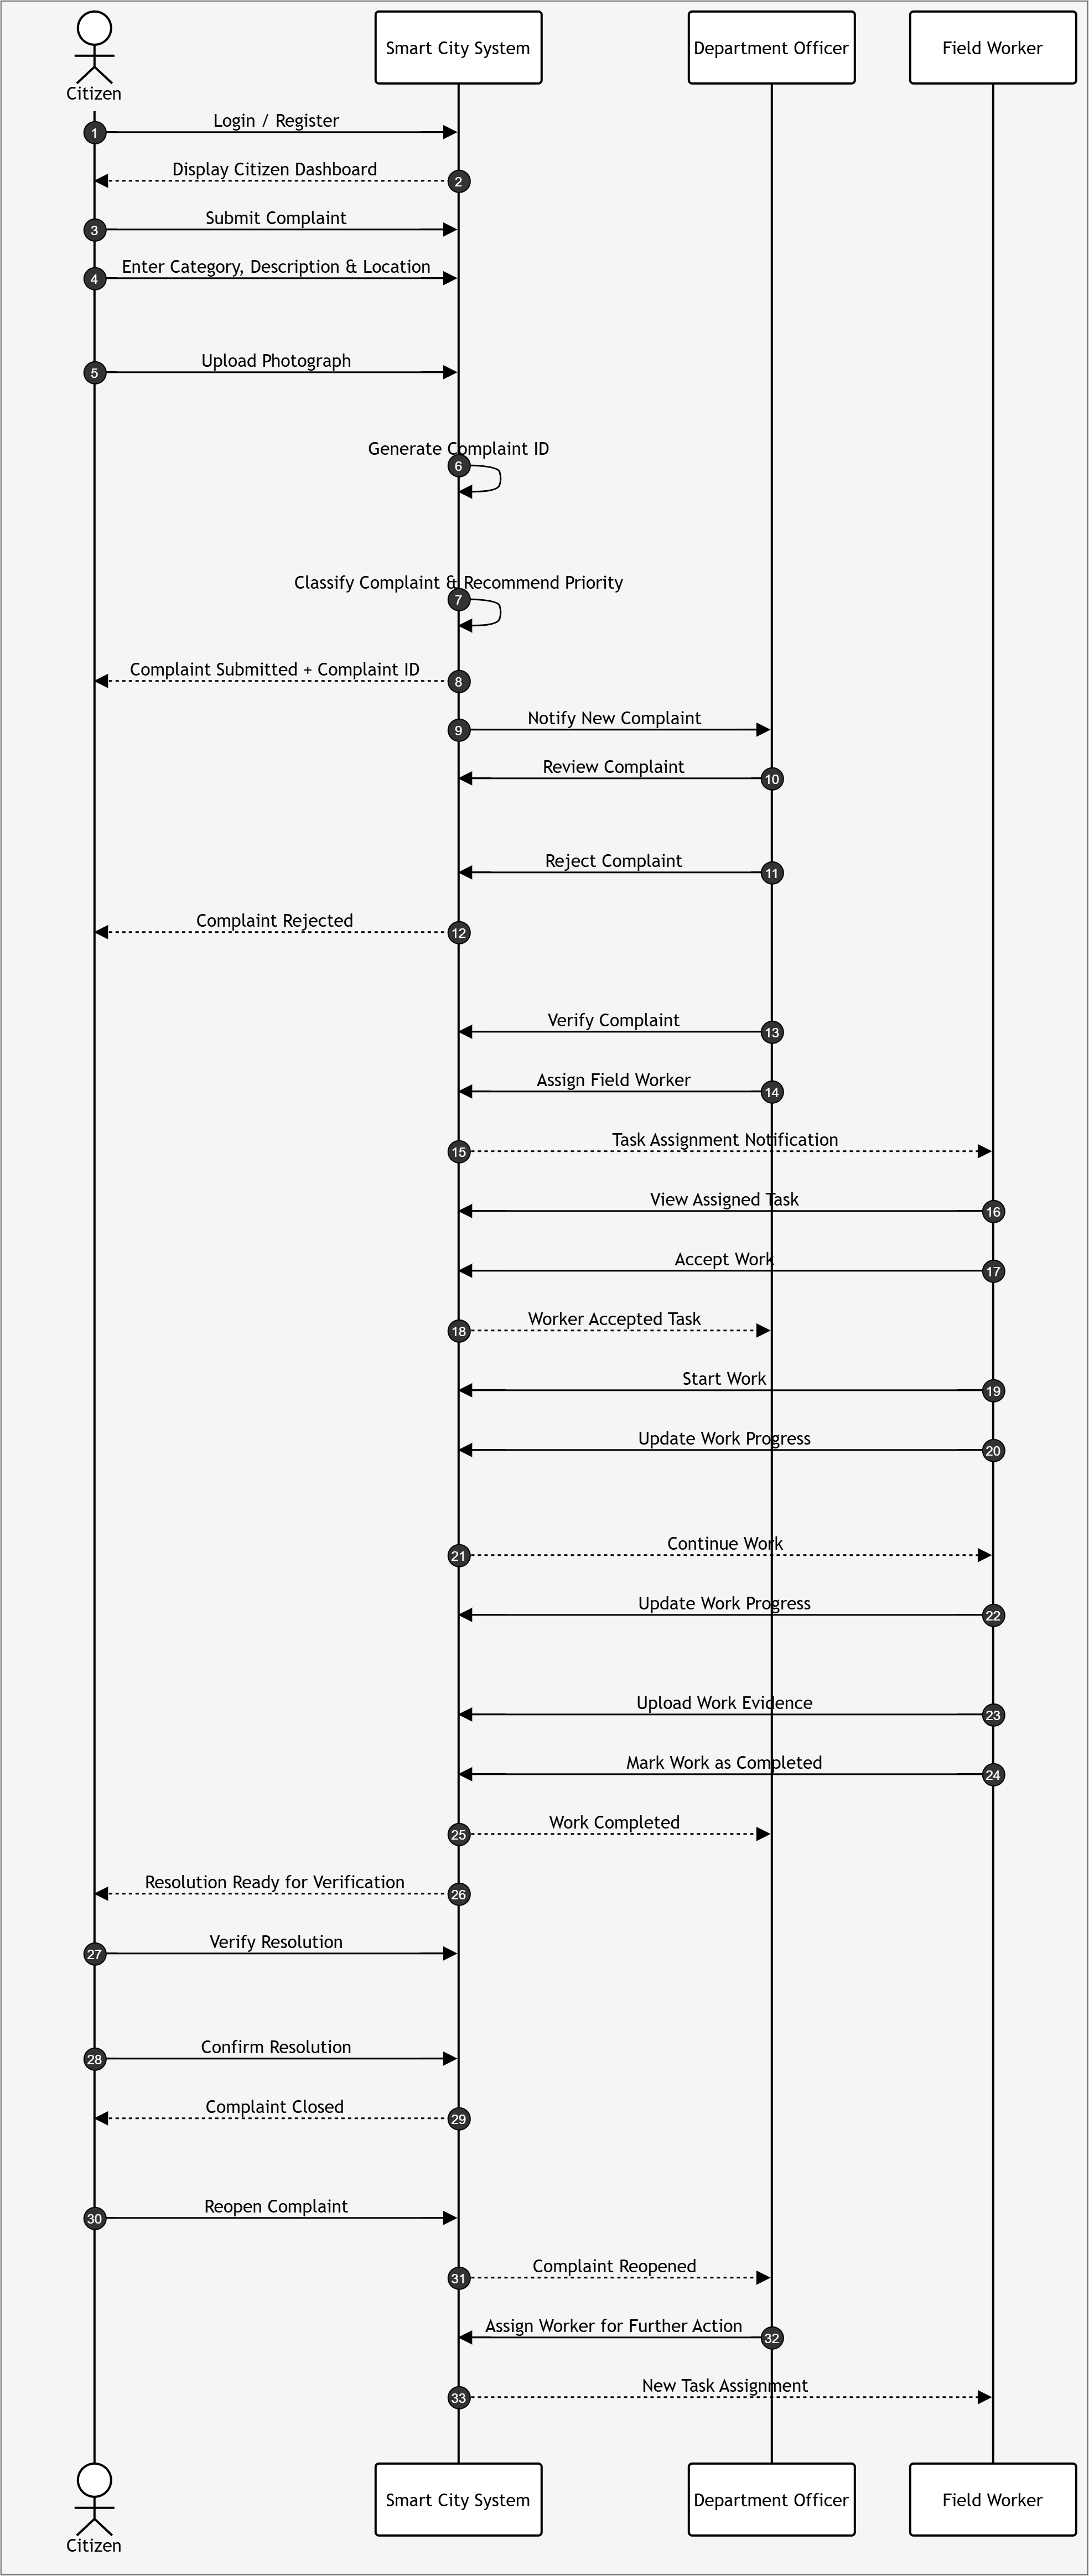
\includegraphics[width=0.60\textwidth]{../assets/Sequence.drawio.png}
    \caption{Sequence Diagram of the Smart City Civic Complaint and Management System}
    \label{fig:sequence}
\end{figure}

% ------------------------------------------------
% SWIMLANE DIAGRAM
% ------------------------------------------------

\subsubsection*{Swimlane Diagram}

The Swimlane Diagram divides the complaint management workflow according to the
responsibility of each participant. It shows which activities are performed by
the Citizen, Smart City System, Department Officer, and Field Worker, making
the distribution of responsibilities clear.

\begin{figure}[H]
    \centering
    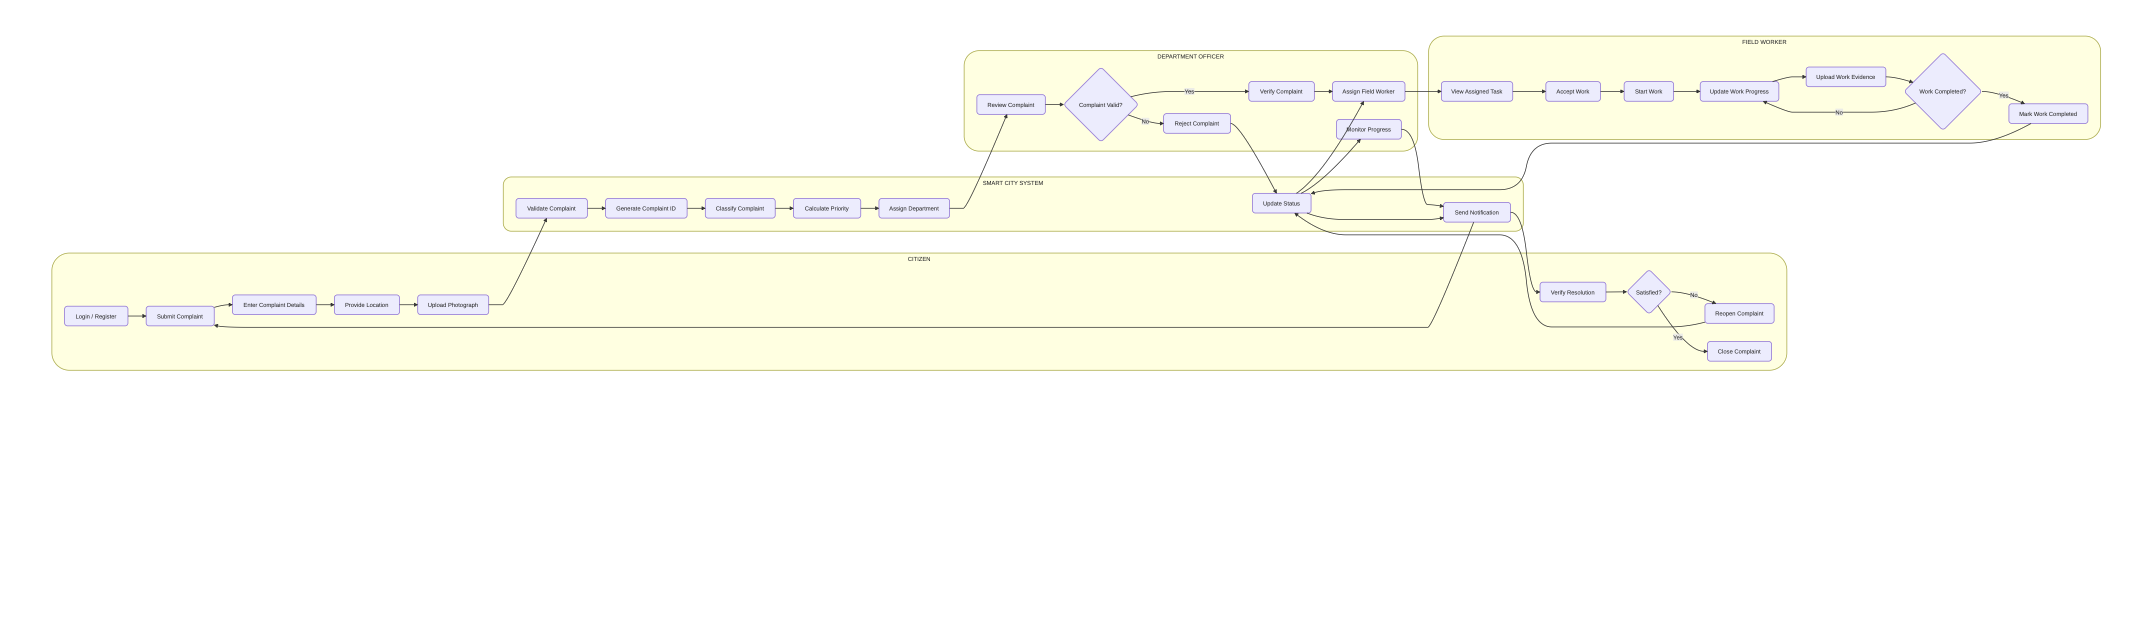
\includegraphics[width=0.90\textwidth]{../assets/Swimlane.png}
    \caption{Swimlane Diagram of the Smart City Civic Complaint and Management System}
    \label{fig:swimlane}
\end{figure}
% ------------------------------------------------
% COLLABORATION DIAGRAM
% ------------------------------------------------

\subsubsection*{Collaboration Diagram}

The Collaboration Diagram represents the interaction and communication between the major objects involved in the complaint management system. It focuses on the messages exchanged between the Citizen, Smart City System, Department Officer, and Field Worker to complete the complaint lifecycle.

\begin{figure}[H]
    \centering
    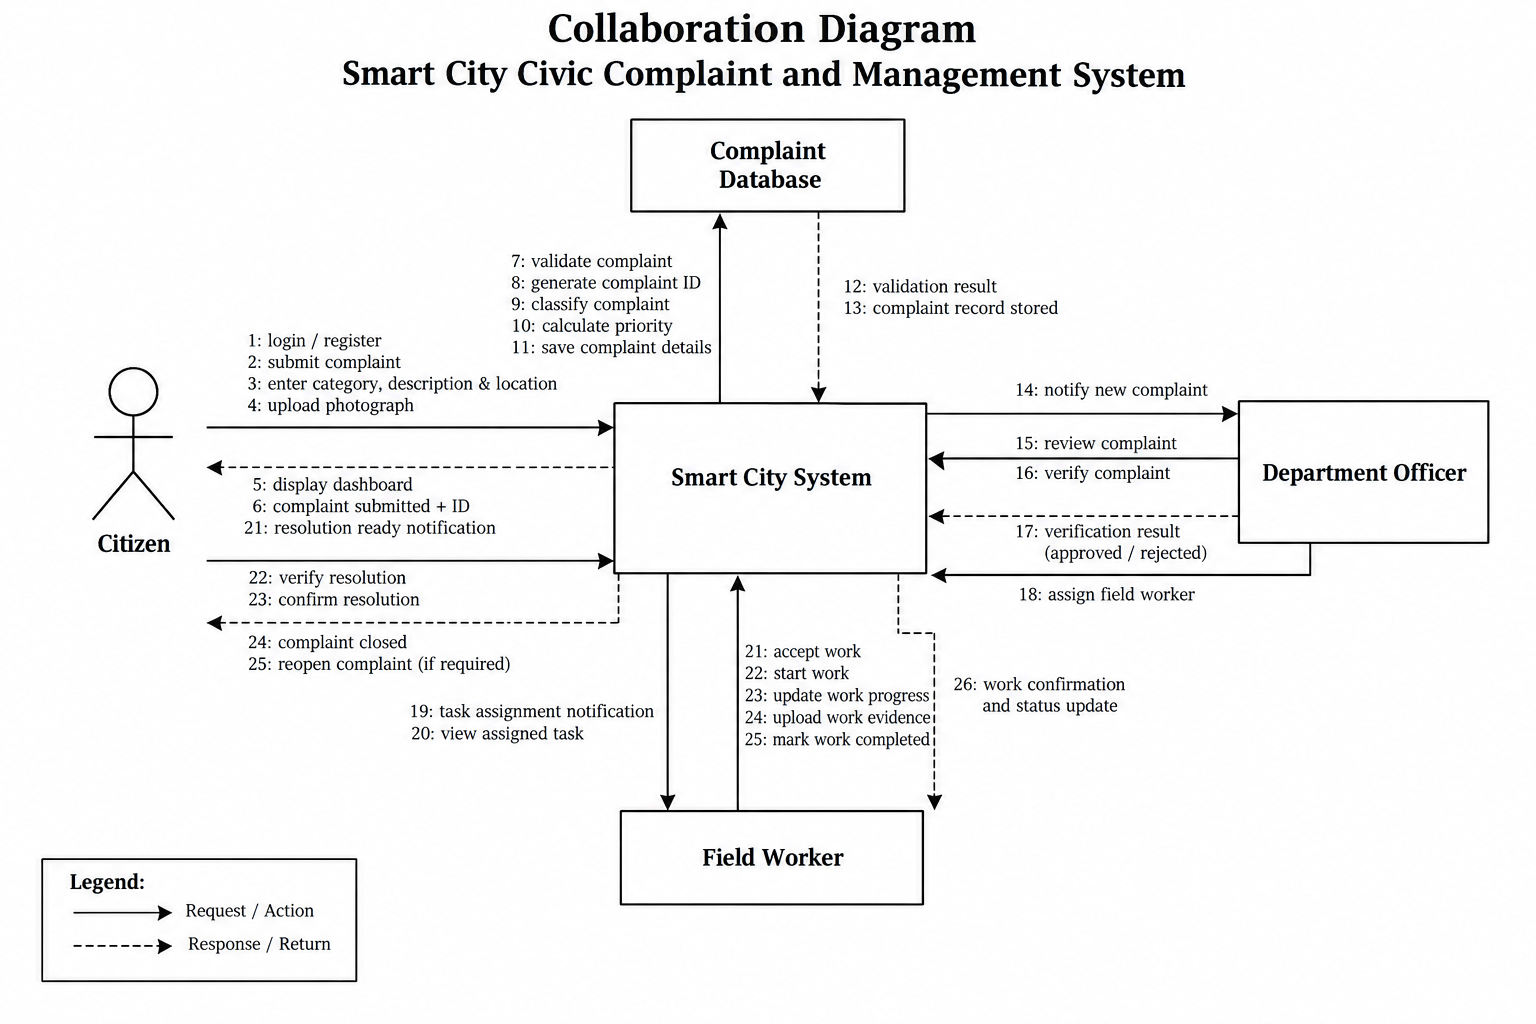
\includegraphics[width=0.90\textwidth]{../assets/Collaboration.png}
    \caption{Collaboration Diagram of the Smart City Civic Complaint and Management System}
    \label{fig:collaboration}
\end{figure}


\subsection{Technical Stack}

The project is being developed as a web-based application using technologies suitable for frontend development and subsequent backend integration.

\begin{longtable}{p{0.25\textwidth} p{0.65\textwidth}}

\toprule
\textbf{Technology / Tool} & \textbf{Purpose} \\
\midrule

HTML & Structure and content of the web pages. \\

CSS & Styling, layout, spacing, typography, and visual presentation of the interface. \\

JavaScript & Client-side interaction and dynamic behaviour of the frontend. \\

VS Code & Primary development environment used for writing and managing project files. \\

Git & Version control for maintaining project history and tracking changes. \\

GitHub & Remote repository used for project collaboration and storage. \\

Draw.io & Used for preparing Software Engineering diagrams such as Use Case, Activity, Swimlane, and Collaboration Diagrams. \\

\bottomrule

\end{longtable}

The current implementation primarily focuses on the frontend and the core user interface. Backend functionality and database integration can be incorporated in subsequent development stages.


\section{Implementation Details}

The implementation follows the functional workflow established during the system design phase.

The core implementation is organized around the complaint lifecycle. Instead of treating complaint submission, assignment, work execution, and resolution as independent processes, they are connected through complaint status and a unique complaint identifier.

The major stages of the implementation are:

\begin{enumerate}[leftmargin=*]

\item User registration and login.

\item Complaint submission.

\item Entry of complaint details.

\item Location and photograph submission.

\item Generation of a complaint ID.

\item Complaint review and verification.

\item Assignment of a field worker.

\item Field work and progress updates.

\item Uploading of work evidence.

\item Completion of the assigned work.

\item Citizen verification of the resolution.

\item Closing or reopening of the complaint.

\end{enumerate}

This modular approach allows individual parts of the system to be developed and tested independently while maintaining the overall complaint workflow.


\subsubsection*{2.2.1 Module 1: Core Functionality}

The Core Functionality module provides the main complaint management features
of the Smart City Civic Complaint and Management System. The module supports
different users of the system, including Citizens, Department Officers,
Field Workers, and Administrators. Each user is provided with an appropriate
interface according to their role.

The module covers user authentication, role-based dashboards, complaint
tracking, complaint review, field task management, and overall complaint
monitoring.

\paragraph{User Authentication}

The system provides a login interface through which users can enter their
email address and password. The user can also select the appropriate role,
such as Citizen, Officer, or Field Worker, before logging into the system.
A registration option is also provided for new users.

\begin{figure}[H]
    \centering
    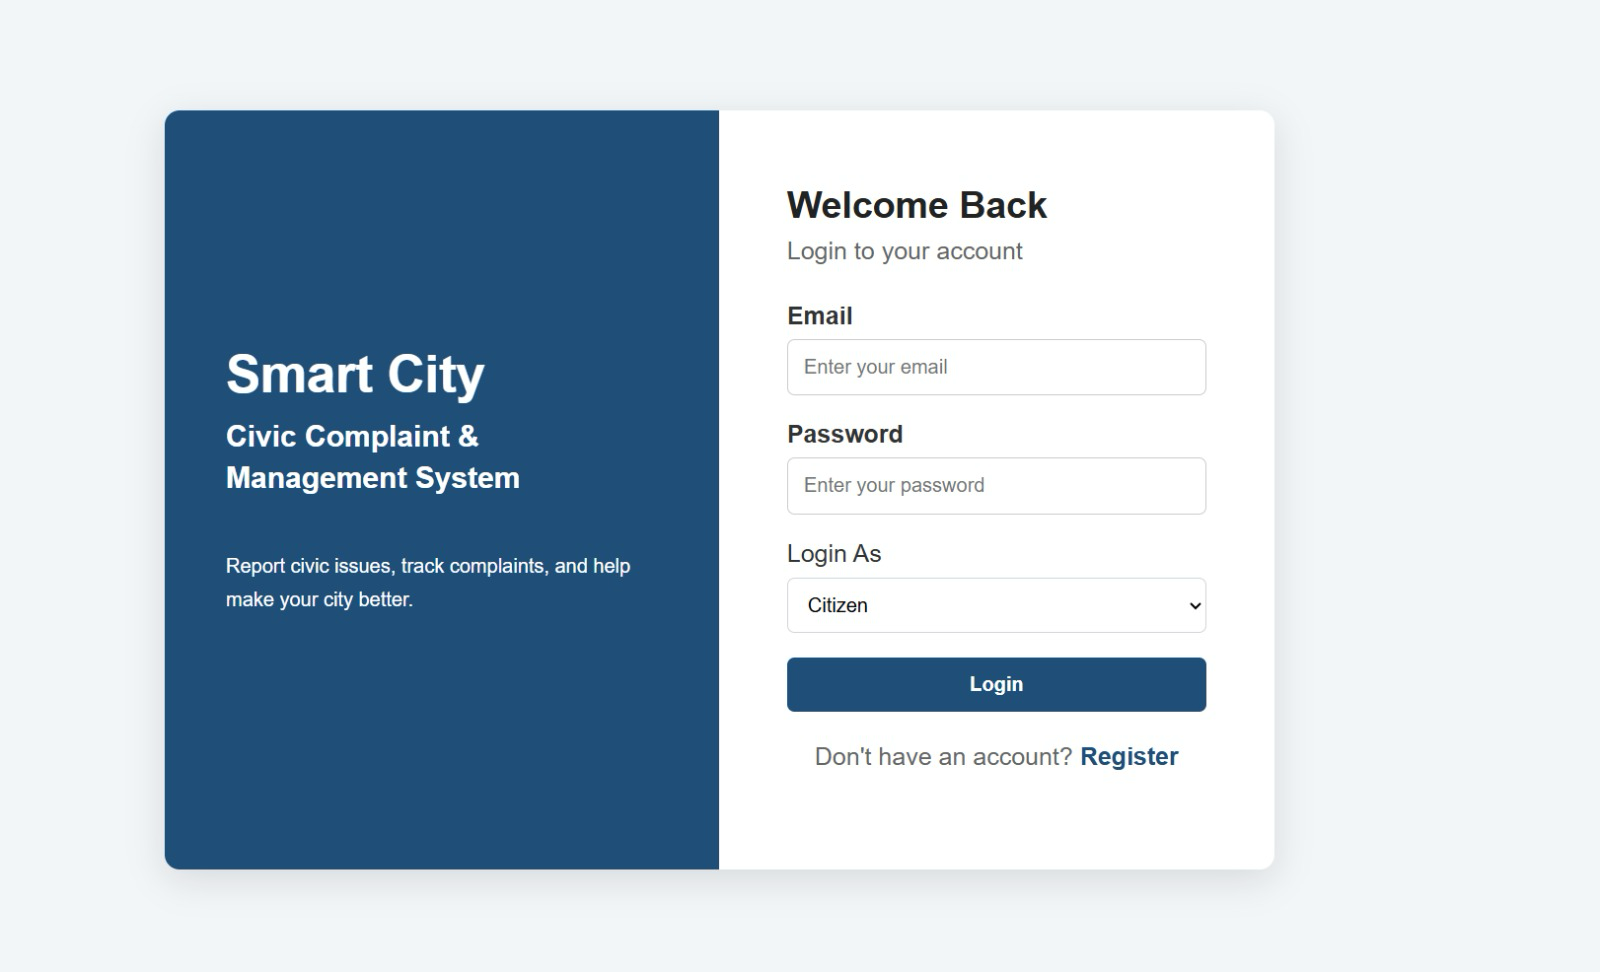
\includegraphics[width=0.90\textwidth]{assets/login.png}
    \caption{User Login Interface}
    \label{fig:login}
\end{figure}

The login interface provides a simple and centralized entry point to the
system. After successful authentication, the user is redirected to the
dashboard corresponding to their selected role.

\paragraph{Citizen Dashboard}

The Citizen Dashboard provides an overview of the complaints submitted by
the citizen. It displays the total number of complaints along with their
current status, including pending, in-progress, and resolved complaints.
The dashboard also provides an option to submit a new complaint and displays
recent complaints for quick access.

\begin{figure}[H]
    \centering
    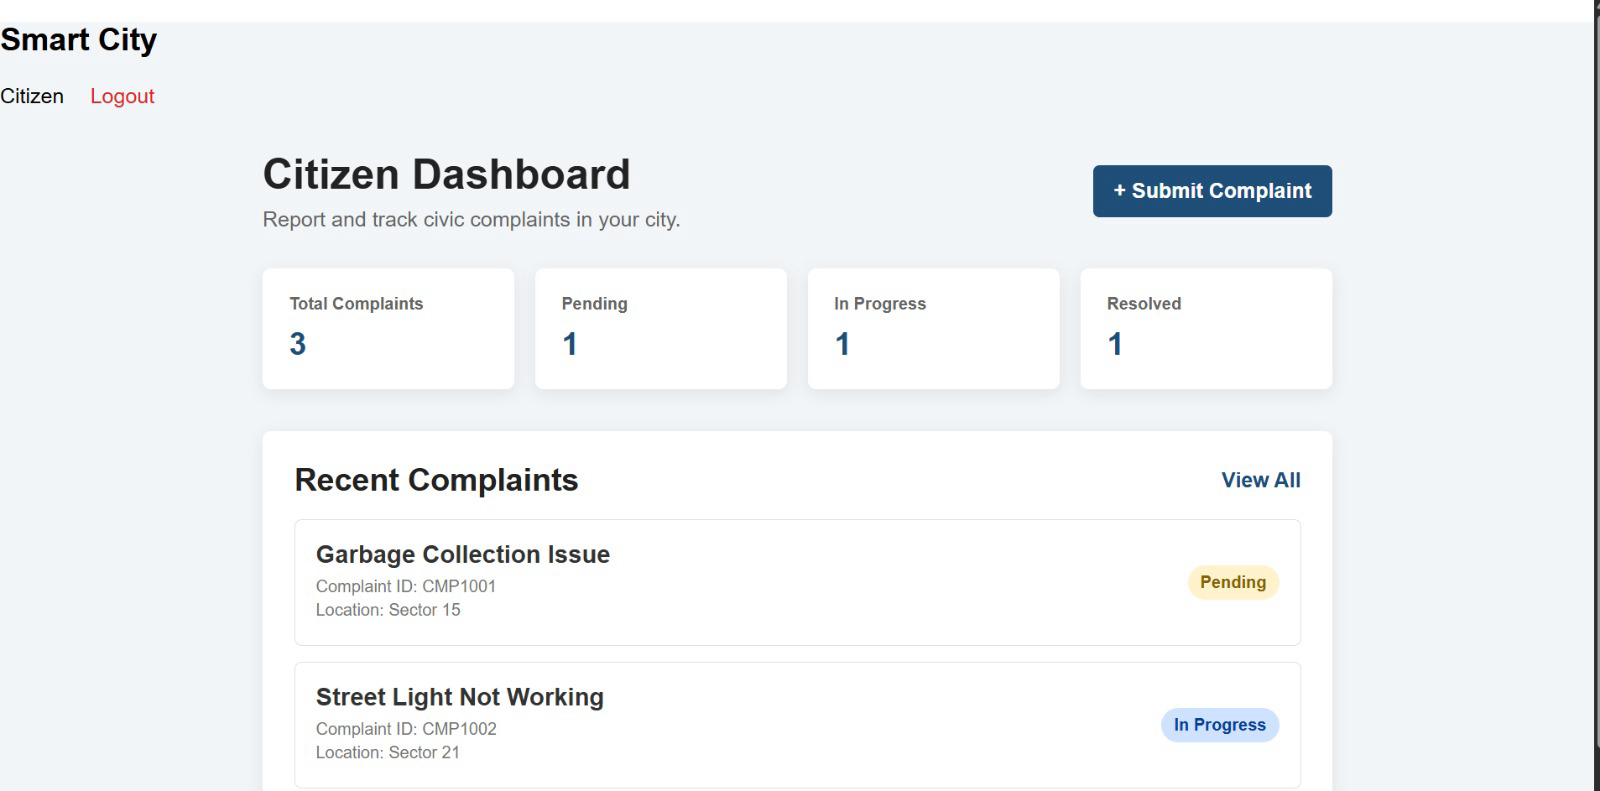
\includegraphics[width=0.90\textwidth]{assets/citizen_dashboard.png}
    \caption{Citizen Dashboard}
    \label{fig:citizendashboard}
\end{figure}

The dashboard allows citizens to monitor their complaints without requiring
them to repeatedly contact the concerned department. The recent complaints
section displays important information such as the complaint title,
complaint ID, location, and current status.

\paragraph{Complaint Tracking}

Citizens can access the ``My Complaints'' section to view all complaints
submitted through the system. Each complaint displays its complaint ID,
category, location, submission date, and current status. A ``View Details''
option allows the citizen to inspect an individual complaint.

\begin{figure}[H]
    \centering
    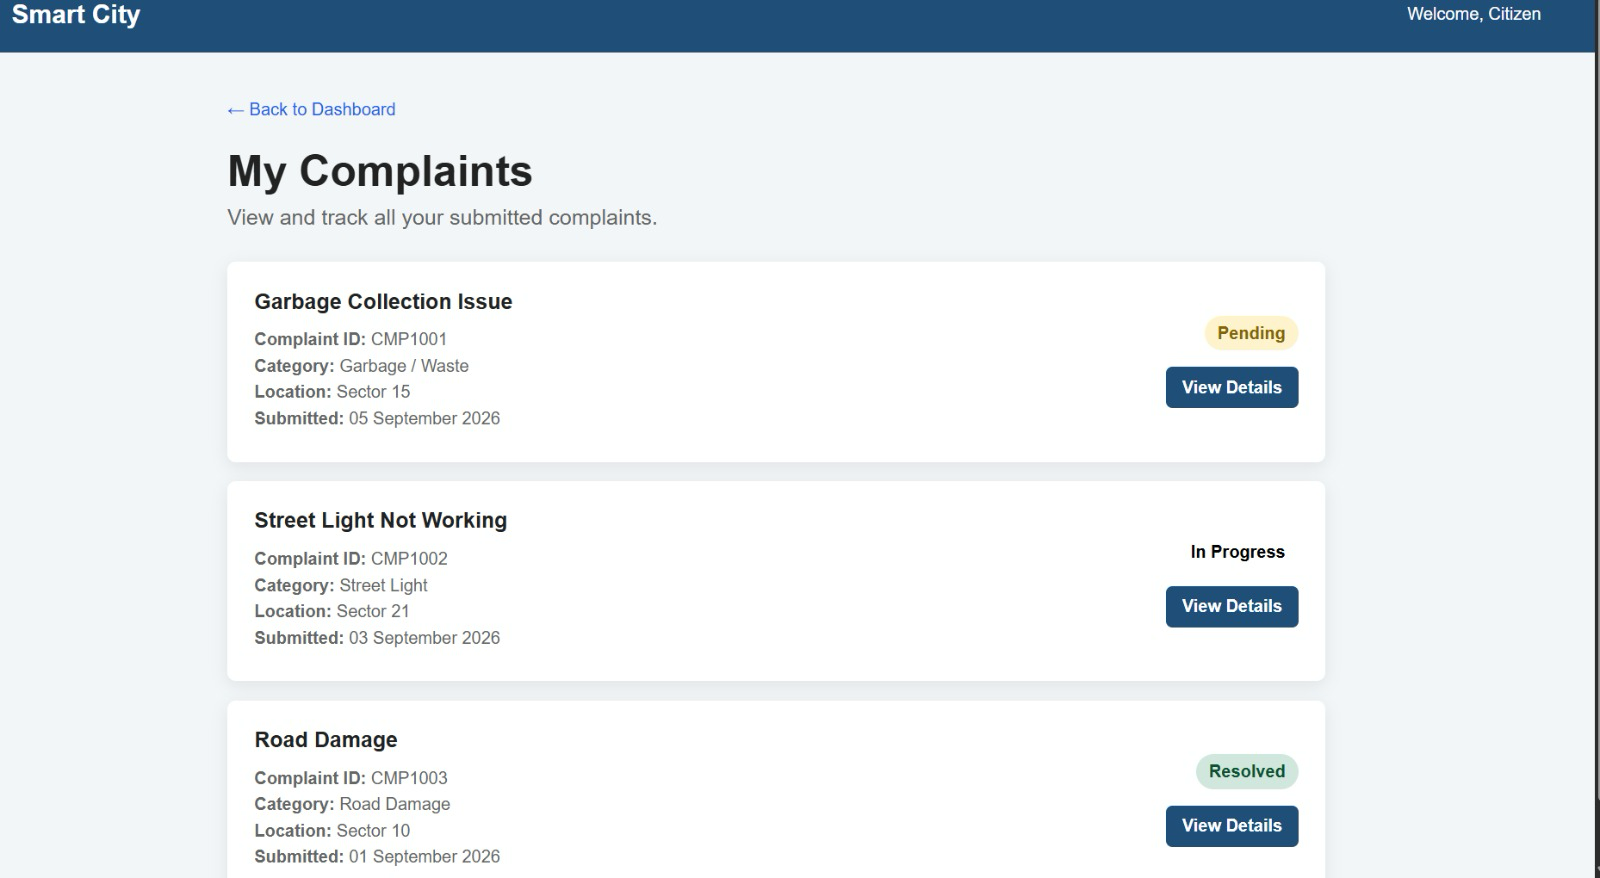
\includegraphics[width=0.90\textwidth]{assets/my_complaints.png}
    \caption{Citizen My Complaints Interface}
    \label{fig:mycomplaints}
\end{figure}

The complaint details interface provides more detailed information about a
selected complaint. It displays the complaint title, complaint ID, category,
location, submission date, status, description, and complaint timeline.

\begin{figure}[H]
    \centering
    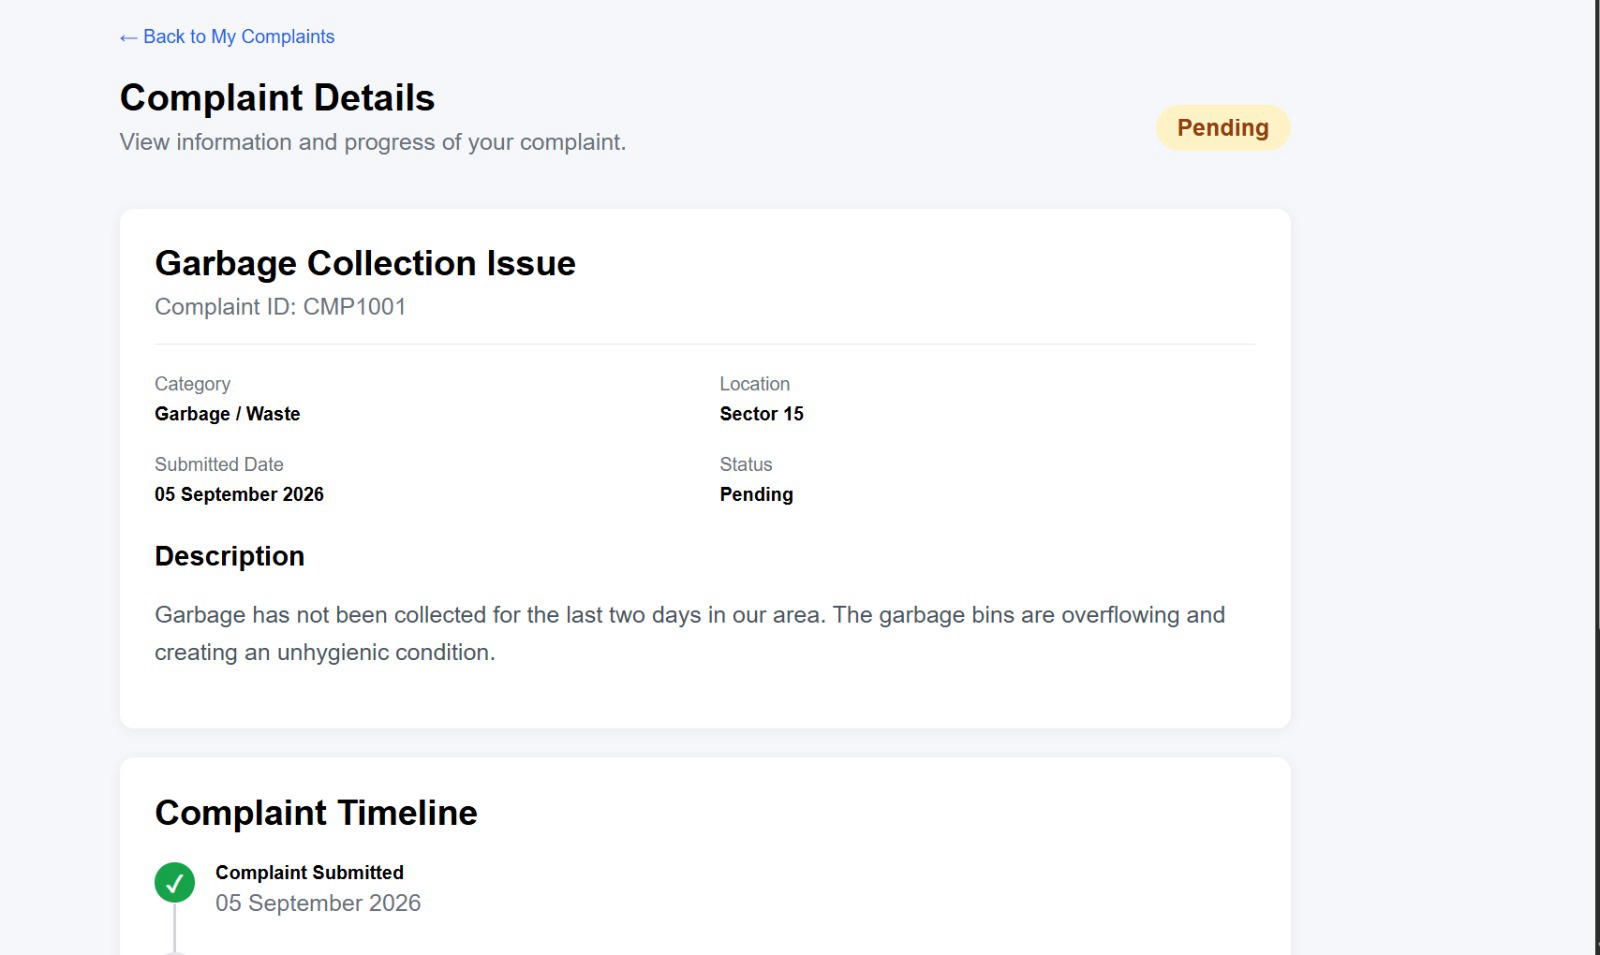
\includegraphics[width=0.90\textwidth]{assets/complaint_details.png}
    \caption{Complaint Details and Status Interface}
    \label{fig:complaintdetails}
\end{figure}

This functionality enables citizens to track the progress of their submitted
complaints and view the current state of the complaint management process.

\paragraph{Department Officer Dashboard}

The Department Officer Dashboard is designed for reviewing and managing
citizen complaints. It provides a summary of total complaints, pending
verification, complaints in progress, and resolved complaints.

\begin{figure}[H]
    \centering
    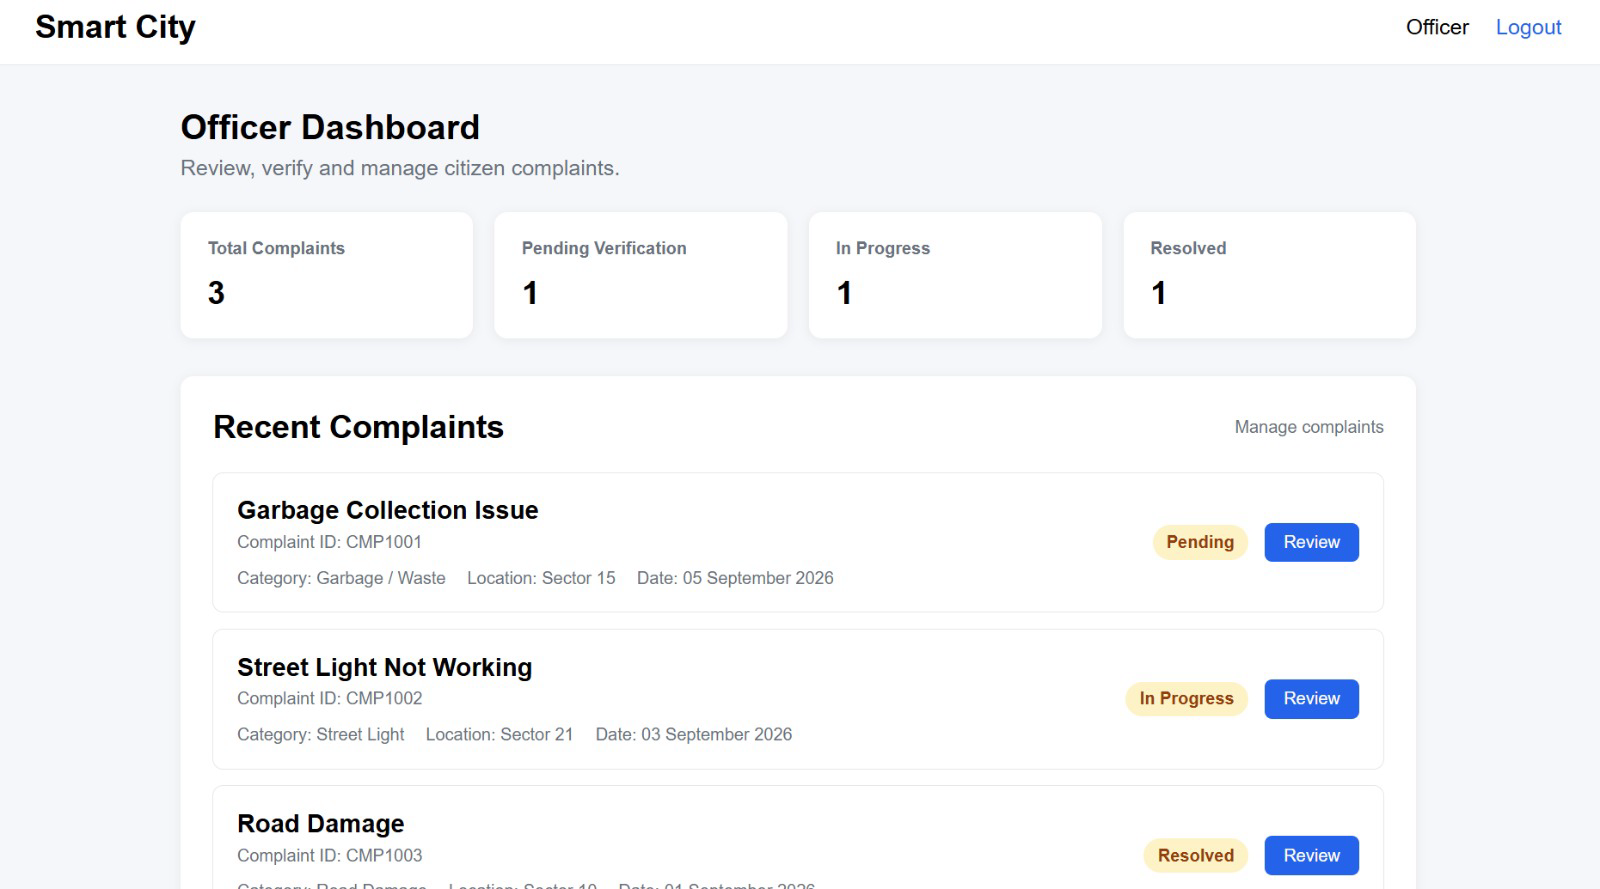
\includegraphics[width=0.90\textwidth]{assets/officer_dashboard.png}
    \caption{Department Officer Dashboard}
    \label{fig:officerdashboard}
\end{figure}

The dashboard also provides a list of recent complaints. The officer can
select a complaint and use the review functionality to inspect the complaint
before taking further action.

\paragraph{Complaint Review}

The complaint review interface allows the Department Officer to examine the
details of a submitted complaint. Information such as the complaint ID,
category, location, submitted date, citizen information, email, status, and
description is displayed.

\begin{figure}[H]
    \centering
    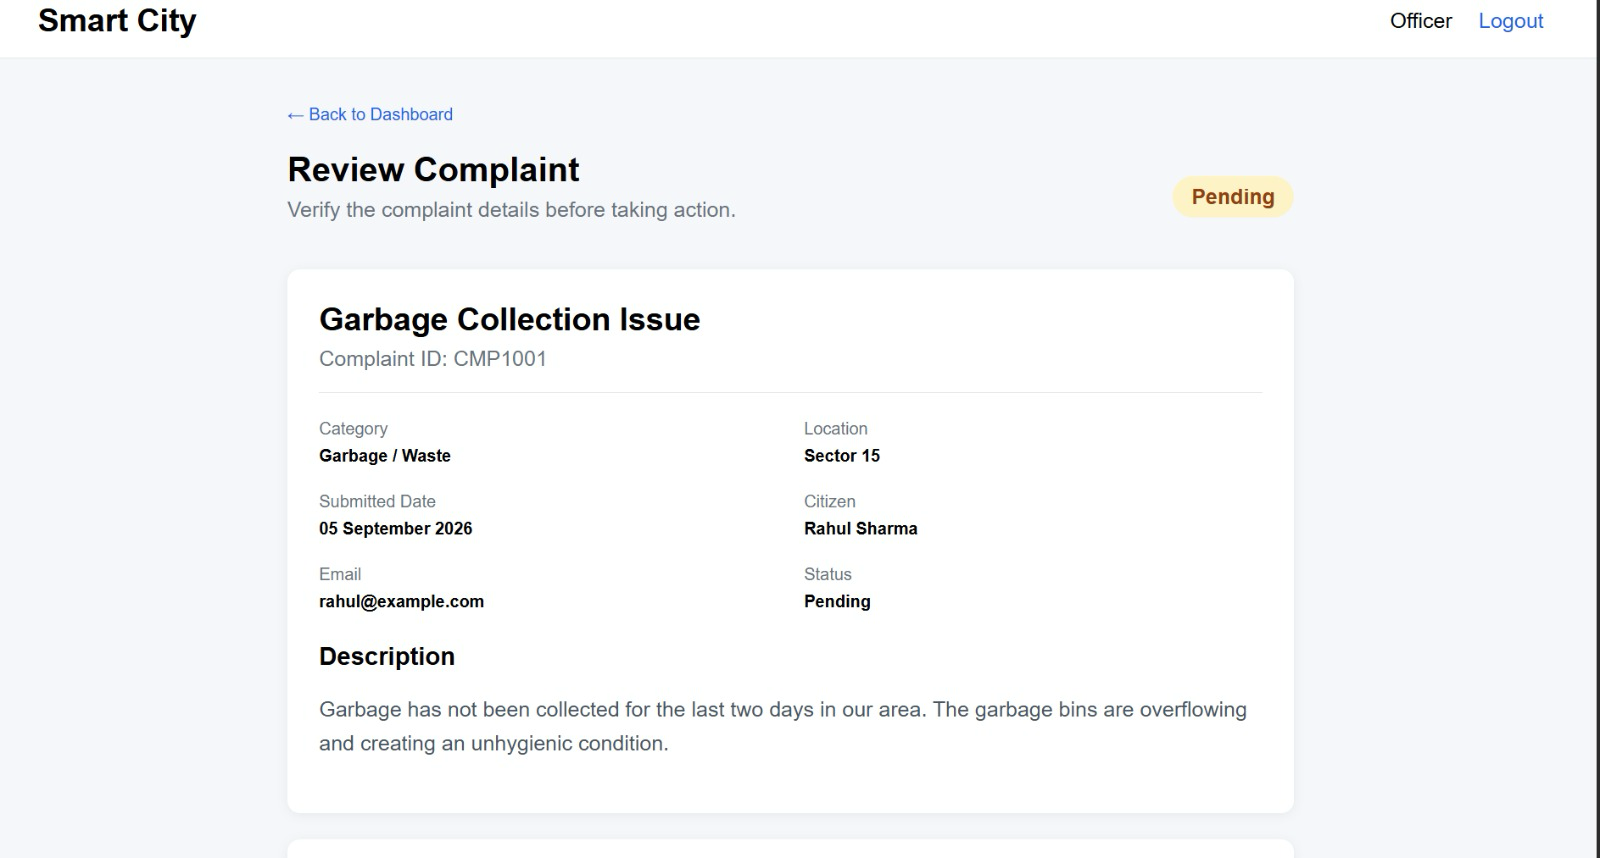
\includegraphics[width=0.90\textwidth]{assets/review_complaint.png}
    \caption{Department Officer Complaint Review Interface}
    \label{fig:reviewcomplaint}
\end{figure}

This functionality provides the officer with the information required to
verify and manage a complaint before it is processed further.

\paragraph{Field Worker Dashboard}

The Field Worker Dashboard provides field workers with an overview of the
complaints or tasks assigned to them. The dashboard displays the number of
assigned tasks, tasks currently in progress, and completed tasks.

\begin{figure}[H]
    \centering
    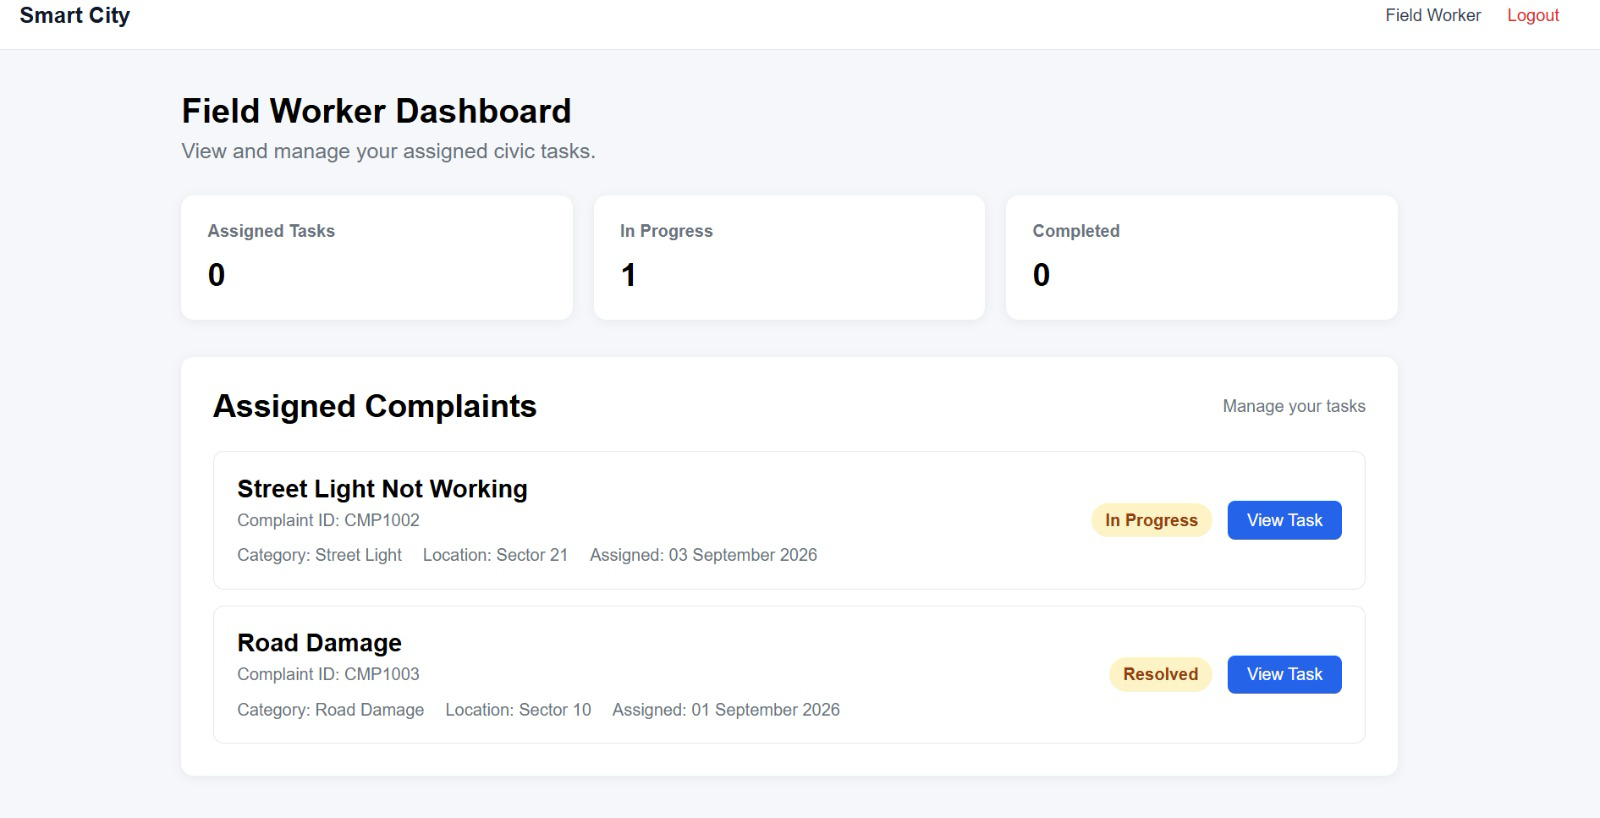
\includegraphics[width=0.90\textwidth]{assets/field_worker_dashboard.png}
    \caption{Field Worker Dashboard}
    \label{fig:fieldworkerdashboard}
\end{figure}

The assigned complaints section provides information such as the complaint
title, complaint ID, category, location, assigned date, and current status.
The field worker can open an assigned task to view its complete details.

\paragraph{Task Management}

The Task Details interface provides the field worker with information about
the assigned complaint. It displays the category, location, assigned date,
assigned authority, current status, and complaint description.

\begin{figure}[H]
    \centering
    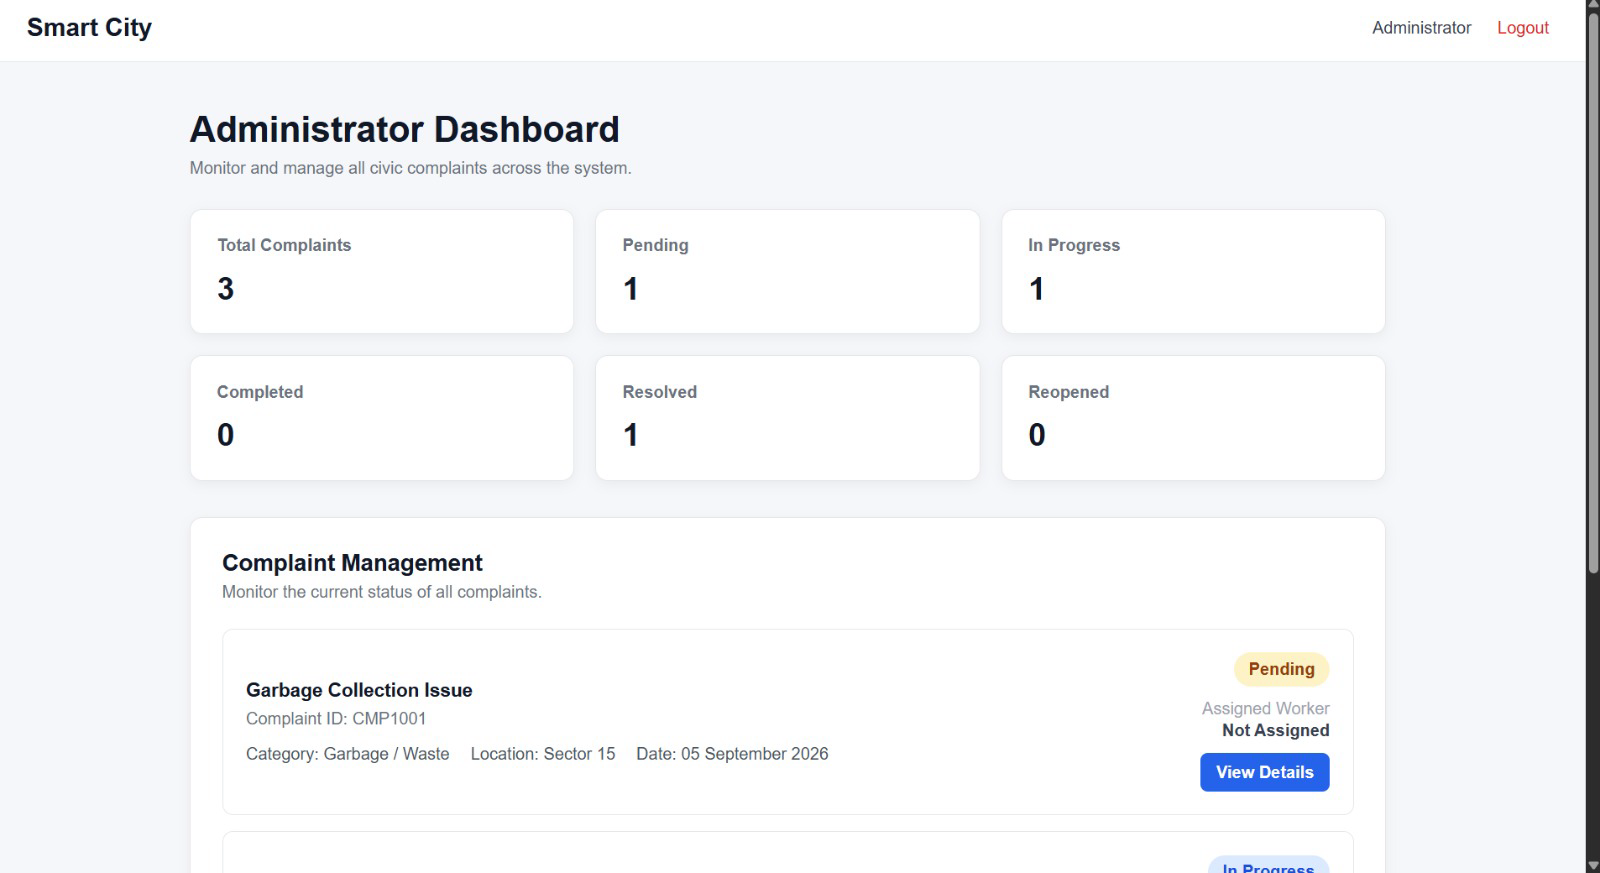
\includegraphics[width=0.90\textwidth]{assets/task_details.png}
    \caption{Field Worker Task Details Interface}
    \label{fig:taskdetails}
\end{figure}

The interface also contains a Worker Action section through which the field
worker can update the progress of the assigned work. This supports the
transition of a complaint from assignment to field-level resolution.

\paragraph{Administrator Dashboard}

The Administrator Dashboard provides an overall view of complaints across
the system. It displays complaint statistics such as total complaints,
pending complaints, complaints in progress, completed complaints, resolved
complaints, and reopened complaints.

\begin{figure}[H]
    \centering
    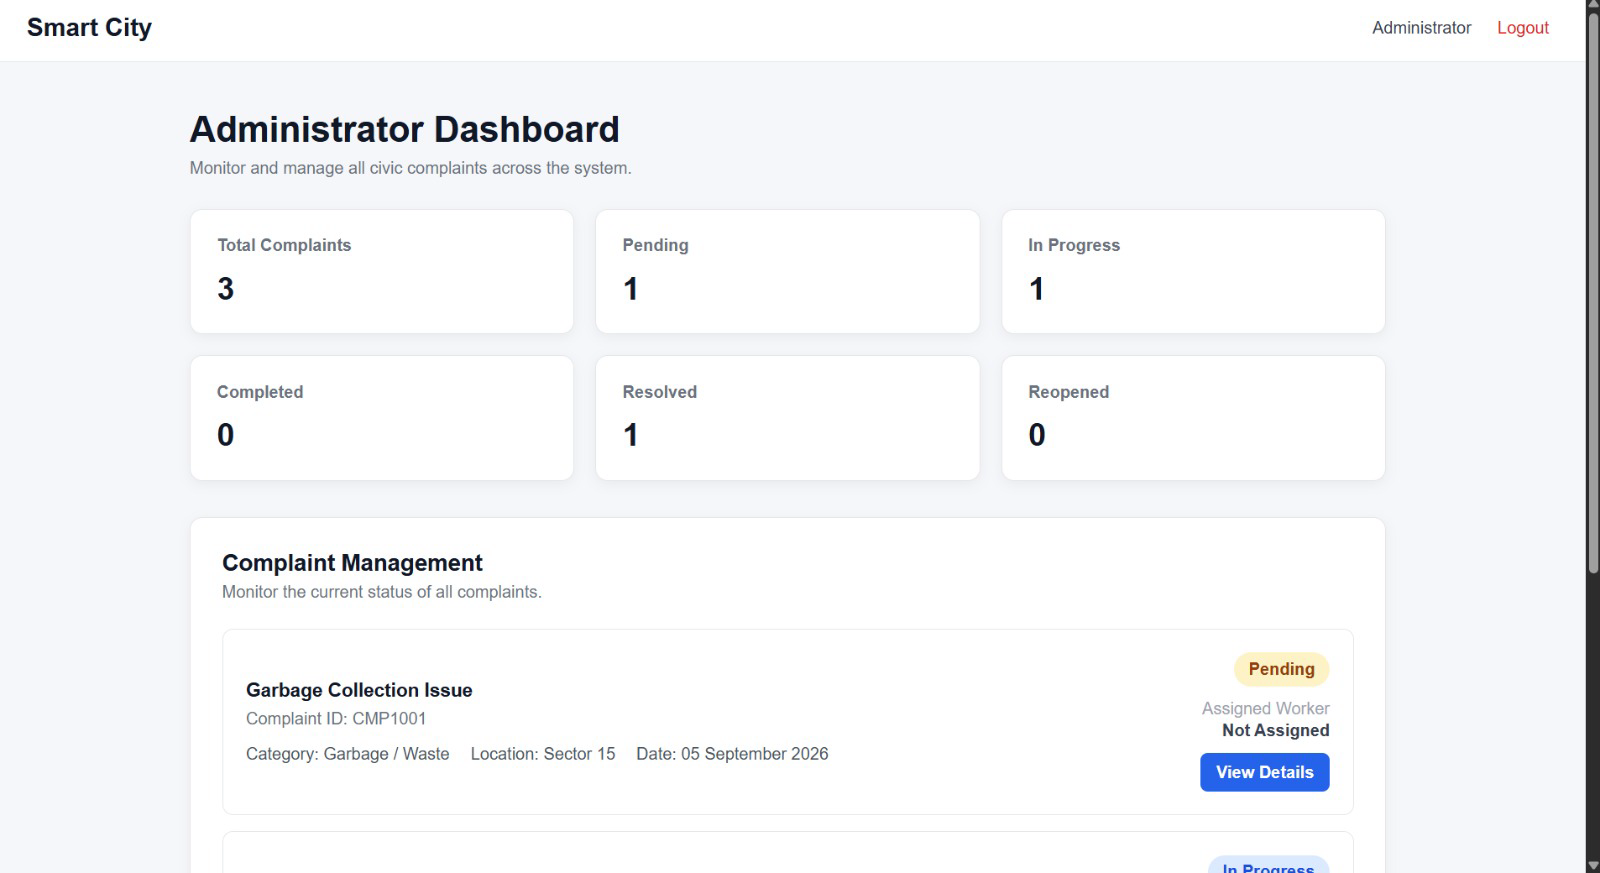
\includegraphics[width=0.90\textwidth]{assets/admin_dashboard.png}
    \caption{Administrator Dashboard}
    \label{fig:admindashboard}
\end{figure}

The complaint management section allows the administrator to monitor the
current status of complaints and view information such as complaint ID,
category, location, date, and assigned worker.

Overall, the Core Functionality module establishes the main workflow of the
system. A citizen can submit and track complaints, a Department Officer can
review and manage complaints, a Field Worker can handle assigned tasks and
update their progress, and an Administrator can monitor complaints across
the system.

\subsubsection*{Core Complaint Status Flow}

The core module maintains a logical sequence of complaint states:

\[
\text{Submitted}
\rightarrow
\text{Under Review}
\rightarrow
\text{Verified}
\rightarrow
\text{Assigned}
\rightarrow
\text{In Progress}
\rightarrow
\text{Completed}
\rightarrow
\text{Closed}
\]

If the complaint is rejected during verification, it follows the rejection path. Similarly, if the citizen is not satisfied with the resolution, the complaint can be reopened and sent for further action.

The status-based approach provides a traceable representation of the complaint lifecycle and allows the different system actors to understand the current state of a complaint.


\subsubsection*{Frontend Implementation}

The current frontend implementation focuses on presenting the core functionality through separate interfaces for the different users.

The main frontend screens include:

\begin{itemize}[leftmargin=*]

\item Login / Registration page.

\item Citizen dashboard.

\item Complaint submission form.

\item Complaint tracking interface.

\item Department officer complaint management interface.

\item Field worker task interface.

\item Work progress and evidence interface.

\item Resolution verification interface.

\end{itemize}

The frontend is structured so that the interface reflects the responsibilities established in the system design. The citizen interacts mainly with complaint creation and verification, while officer and worker interfaces support the processing and resolution stages.


% =================================================
% END OF REPORT SECTION 2.2.1
% =================================================

\end{document}